\section{Results}
\label{results}
Examining the distribution of sentiments, a definite majority of neutral statements  (69\%) is clearly obvious. The proportion of positive annotated statements (21\%) is about twice as large as the number of negatively annotated terms (11\%). This implies a slight tendency to an overall positive attitude towards the future of AI (\autoref{fig:bar_sentiments}). In \autoref{fig:bar_topics} a domination of neutral statements is illustrated for each of the 9 topics. With two exceptions, \emph{gaming} and \emph{machine human interface}, there are visibly more positive than negative statements on each topic.
\\
\\
When analyzing the topics, we find the statements not being equally distributed among all these categories.
While we divided all statements into the 9 topics, \emph{machine human interface} describes about half of all statements (48\%).
\emph{gaming} as well as \emph{natural language technology} account for about 15\% of all statements (\autoref{fig:pie_topics_by_occ}).
\begin{figure}[t]
    \centering
    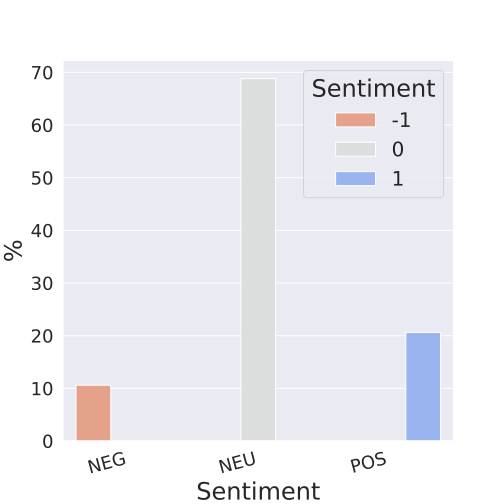
\includegraphics[width=\linewidth]{bar_sentiments}
    \caption{
        \highlight{Dummy caption}.
    }
    \label{fig:bar_sentiments}
\end{figure}
\\
\\
In the distribution of subtopics, we can observe a similar dominance of some subcategories. For instance, the subcategory \emph{data} is associated with 21\% of all statements, as well as \emph{autopilot}. Other dominant subtopics are \emph{intelligence} (19\%), \emph{recognition} (12\%), \emph{computer} (8\%) and \emph{supercomputer} (7\%) (\autoref{fig:pie_subtopics_by_occ}).
\\
\\
As previously described we added for sentiment of every statement.
Calculating the average the sentiment score is about 0.1.
This shows a slightly positive tendency.
The average sentiment of the most topics is majorly neutral.
The categories containing the most positive rated sentiments are \emph{transhumanism}, \emph{natural language technology}, and \emph{research computing}. The most negative sentiment on average were assigned to the categories \emph{gaming} and \emph{search engine}. 3 of the 5 most common subtopics of \emph{gaming} have a sentiment score of less than 0 (\autoref{fig:pie_topics_subtopics_by_occ_sent_neu}).
